\chapter{METODOLOGI}
\label{chap:metodologi}

% Ubah bagian-bagian berikut dengan isi dari desain dan implementasi

Proses pengerjaan dilakukan sesuai dengan desain sistem berikut dan implementasinya. Perancangan sistem adalah konsep pembuatan dan perancangan infrastruktur, yang kemudian diimplementasikan dalam bentuk blok diagram yang dikerjakan.

%Section 3.1
\section{Metode yang digunakan}
\label{sec:deskripsisistem}
Pada penelitian ini diintegrasikan teknologi visi komputer dengan sistem tertanam agar dapat mengontrol gerak kursi roda menggunakan gerakan mata (\emph{eye gesture}). Berikut merupakan blok diagram \emph{software} yang diimplementasikan dalam penelitian ini.

%Gambar 3.1
\begin{figure} [ht] \centering
  % Nama dari file gambar yang diinputkan
  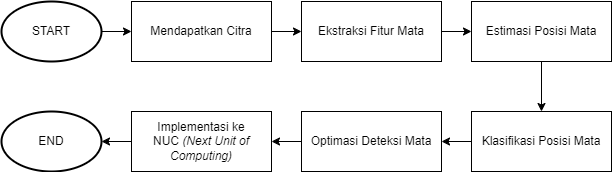
\includegraphics[scale=0.7]{gambar/bab3/software.png}
  % Keterangan gambar yang diinputkan
  \caption{Blok Diagram \textit{Software}}
  % Label referensi dari gambar yang diinputkan
  \label{fig:software}
\end{figure}

\subsection{Mendapatkan Citra}

Dalam mengerjakan penelitian ini, langkah pertama yang dilakukan adalah pengambilan citra menggunakan kamera atau sumber gambar lainnya. Citra yang diambil harus cukup jelas dan terfokus pada area wajah agar fitur mata dapat diidentifikasi dengan akurat. Pengambilan citra dapat dilihat pada Gambar \ref{fig:citra}.\\

%Gambar 3.2
\begin{figure} [ht] \centering
  % Nama dari file gambar yang diinputkan
  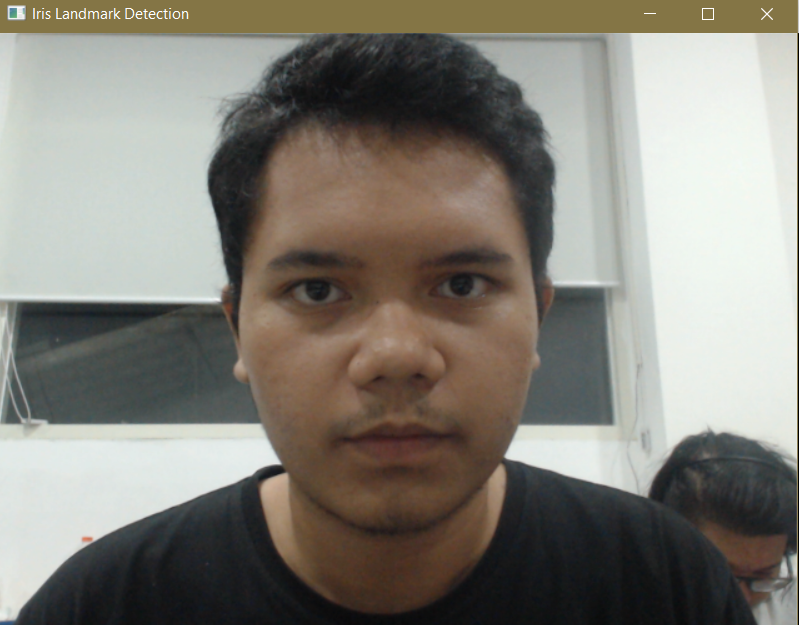
\includegraphics[scale=0.35]{gambar/bab3/citra.png}
  % Keterangan gambar yang diinputkan
  \caption{Pengambilan Citra}
  % Label referensi dari gambar yang diinputkan
  \label{fig:citra}
\end{figure}

\subsection{Ekstraksi Fitur Mata}
Pengenalan pose adalah proses yang melibatkan penggunaan bahasa pemrograman Python, \emph{library} OpenCV, dan \emph{framework} MediaPipe. Dalam konteks ini, Mediapipe berperan penting dalam memperoleh informasi titik \emph{landmark} yang signifikan terhadap objek yang diidentifikasi. \emph{Landmarks} inilah yang menjadi dasar pembentukan representasi visual dari pose tersebut. Proses selanjutnya adalah membuat garis yang menghubungkan titik-titik \emph{landmark} yang diberikan dan menggambarkan hubungan spasial antar titik-titik tersebut. Dengan demikian, metode ini tidak hanya menggunakan Mediapipe Face Mesh sebagai framework utama, tetapi juga  OpenCV sebagai alat analisis gambar dan manipulasi visual yang diperlukan untuk pengenalan gestur mata.

Pada penelitian ini akan digunakan salah satu fitur dari MediaPipe yaitu MediaPipe Face Mesh. MediaPipe Face Mesh memiliki cara kerja yang sama dengan MediaPipe, namun MediaPipe Face Mesh secara khusus dibuat untuk mengidentifikasi area wajah manusia. Untuk semua \textit{landmark} yang tersedia pada MediaPipe Face Mesh dapat dilihat pada Gambar \ref{fig:landmark}.

% Gambar 3.3
\begin{figure} [ht] \centering
  % Nama dari file gambar yang diinputkan
  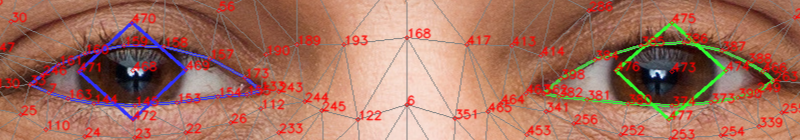
\includegraphics[scale=0.07]{gambar/landmark.png}
  % Keterangan gambar yang diinputkan
  \caption{Arsitektur pada MediaPipe Face Mesh \textit{Landmarks}}
  % Label referensi dari gambar yang diinputkan
  \label{fig:landmark}
\end{figure}

Proses pengerjaan penelitian ini akan memanfaatkan teknologi \emph{eye pose detection} dari MediaPipe Face Mesh untuk mengontrol gerak kursi roda. Terdapat beberapa titik yang dibagi menjadi 4 kelas yaitu LEFT\_EYE (kelopak mata sebelah kiri), LEFT\_IRIS (iris mata sebelah kiri), RIGHT\_EYE (kelopak mata sebelah kiri), dan RIGHT\_IRIS (iris mata sebelah kiri). Titik-titik tersebut atau yang disebut dengan \emph{keypoints} akan digunakan pada estimasi posisi. Titik-titik \emph{keypoints} yang digunakan pada estimasi posisi ini dapat dilihat pada Tabel \ref{tbl:titik keypoints}.

% Tabel 3.1
\begin{table}[H]
\centering
    \caption{Tabel Titik \emph{Keypoints} yang Relevan pada Tahap Estimasi Posisi Kelopak Mata dan Iris Mata}
    \label{tbl:titik keypoints}
    \begin{tabular}{|c|c|}                                                                        
     \hline
      Nama        & Keypoints                                                       \\ 
      \hline
      LEFT\_EYE   &362,382,381,380,374,373,390,249,263,466,388,387,386,385,384,398  \\ 
      \hline
      LEFT\_IRIS  &474,475,476,477                                                  \\ 
      \hline
      RIGHT\_EYE  &33,7,163,144,145,153,154,155,133,173,157,158,159,160,161,246    \\ 
      \hline
      RIGHT\_IRIS &469,470,471,472                                                  \\     
      \hline
    \end{tabular}
\end{table}

\subsection{Estimasi Posisi Mata}

Proses estimasi posisi mata dilakukan dengan mendeteksi keberadaan mata pada citra yang didapatkan. Setelah posisi mata didapatkan, selanjutnya dilakukan deteksi untuk 40 titik landmark pada bagian kelopak mata dan iris mata. Untuk melakukan estimasi posisi mata, beberapa titik \emph{landmark} yang terdapat pada Tabel \ref{tbl:titik keypoints} akan digambarkan dan diwarnai dengan warna yang unik untuk membantu membedakan setiap bagian mata. Secara spesifik, warna yang diberikan pada setiap titik \emph{landmark} mencerminkan hubungan dengan bagian mata tertentu, sehingga memberikan representasi visual yang detail dan informatif.

Proses ini sangat penting dalam aplikasi pengenalan wajah dan analisis visual, di mana keakuratan dalam mengidentifikasi dan memetakan titik-titik penting pada mata dapat secara signifikan meningkatkan efektivitas sistem. Melalui pendekatan ini, sistem dapat lebih mudah memahami orientasi dan posisi mata dalam berbagai kondisi pencahayaan dan sudut pandang, memastikan hasil yang lebih \emph{robust} dan akurat.Untuk lebih jelasnya berikut contoh gambar dengan estimasi posisi mata yang dapat dilihat pada Gambar \ref{fig:contoh citra yang telah diestimasi pose}. 

% Gambar 3.4
\begin{figure} [ht] \centering
    % Nama dari file gambar yang diinputkan
    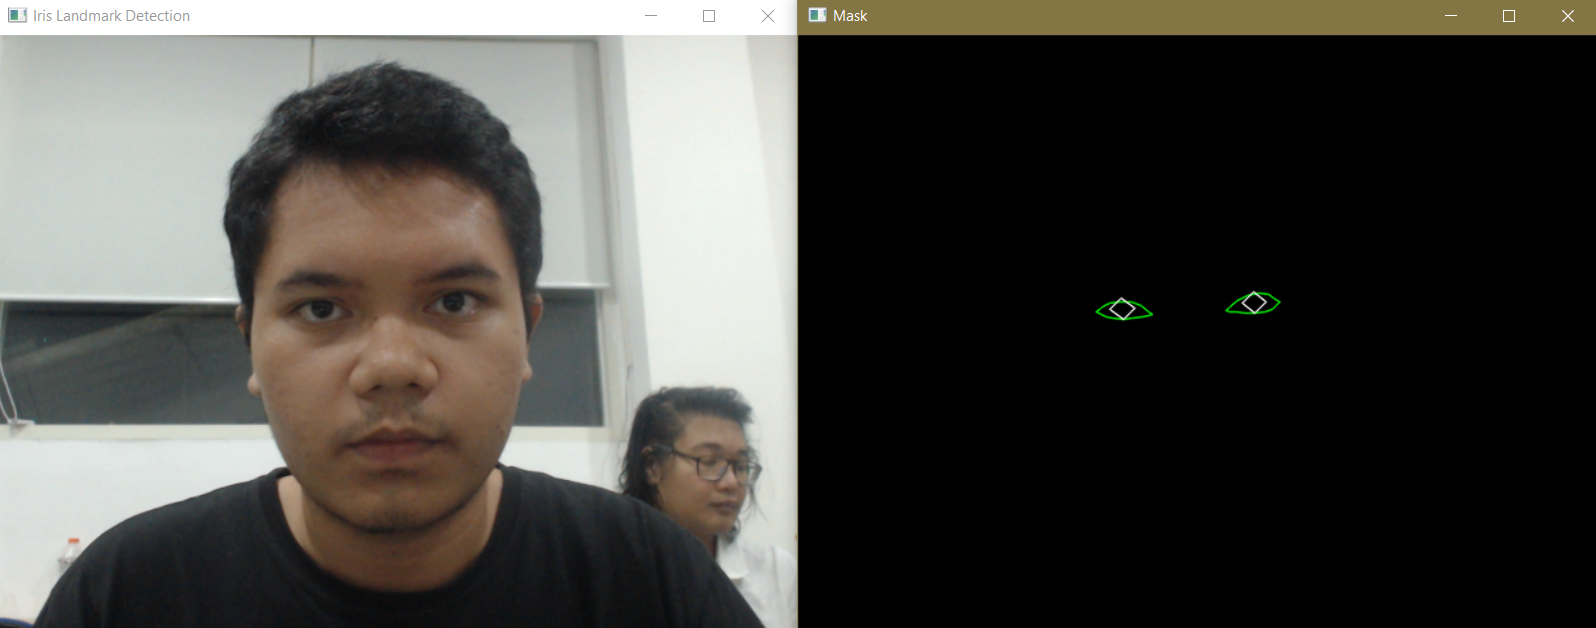
\includegraphics[scale=0.35]{gambar/bab3/iris.png}
    % Keterangan gambar yang diinputkan
    \caption{Citra yang Telah Diestimasi Posisi Kelopak Mata dan Iris Mata}
    % Label referensi dari gambar yang diinputkan
    \label{fig:contoh citra yang telah diestimasi pose}
\end{figure}


\subsection{Klasifikasi Posisi Mata}
Setelah proses estimasi posisi mata selesai, maka langkah selanjutnya ada mengelompokkan citra-citra hasil estimasi ke dalam dataset. Dataset ini akan memiliki 3 kelas berbeda, mewakili perintah untuk bergerak ke kanan, bergerak ke kiri, dan berhenti. Kelas ini mewakili perintah dasar untuk menggerakkan kursi roda. 

Pengelompokan ini memungkinkan sistem untuk mempelajari dan memahami pola-pola gerakan mata yang berkaitan dengan masing-masing perintah, sehingga memfasilitasi pengembangan algoritma yang dapat secara efektif menerjemahkan isyarat visual menjadi aksi nyata. Dengan demikian, penggunaan dataset yang terstruktur dan tersegmentasi secara khusus ini sangat krusial dalam meningkatkan keakuratan respons kursi roda terhadap perintah yang diberikan oleh pengguna.

% Tabel 3.2
\begin{table}[H]
\centering
    \caption{Tabel Contoh Klasifikasi Citra}
    \label{tbl:contoh-klasifikasi}
    \begin{tabular}{|c|c|}
        \hline
        Posisi              & Citra              \\ \hline
        Kanan                & 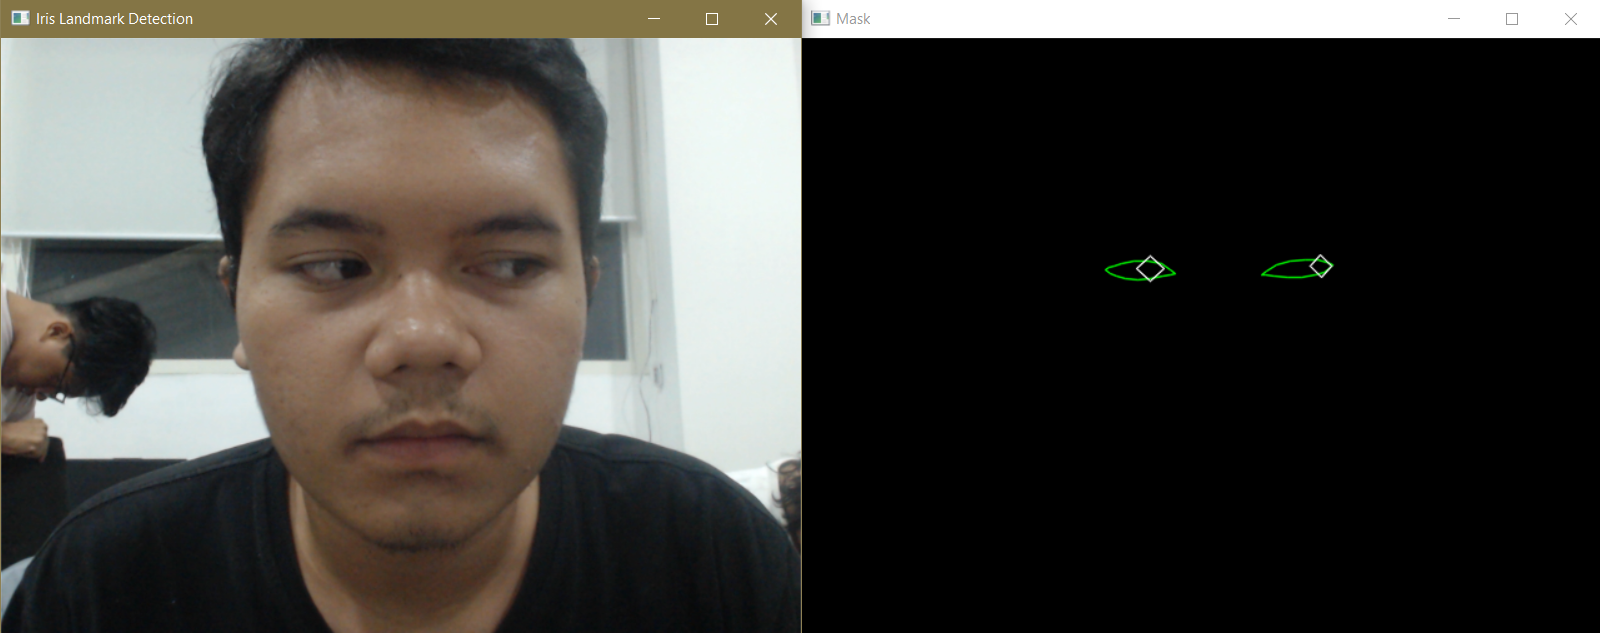
\includegraphics[scale=0.25]{gambar/bab3/kanan.png}   \\ \hline
        Kiri                & 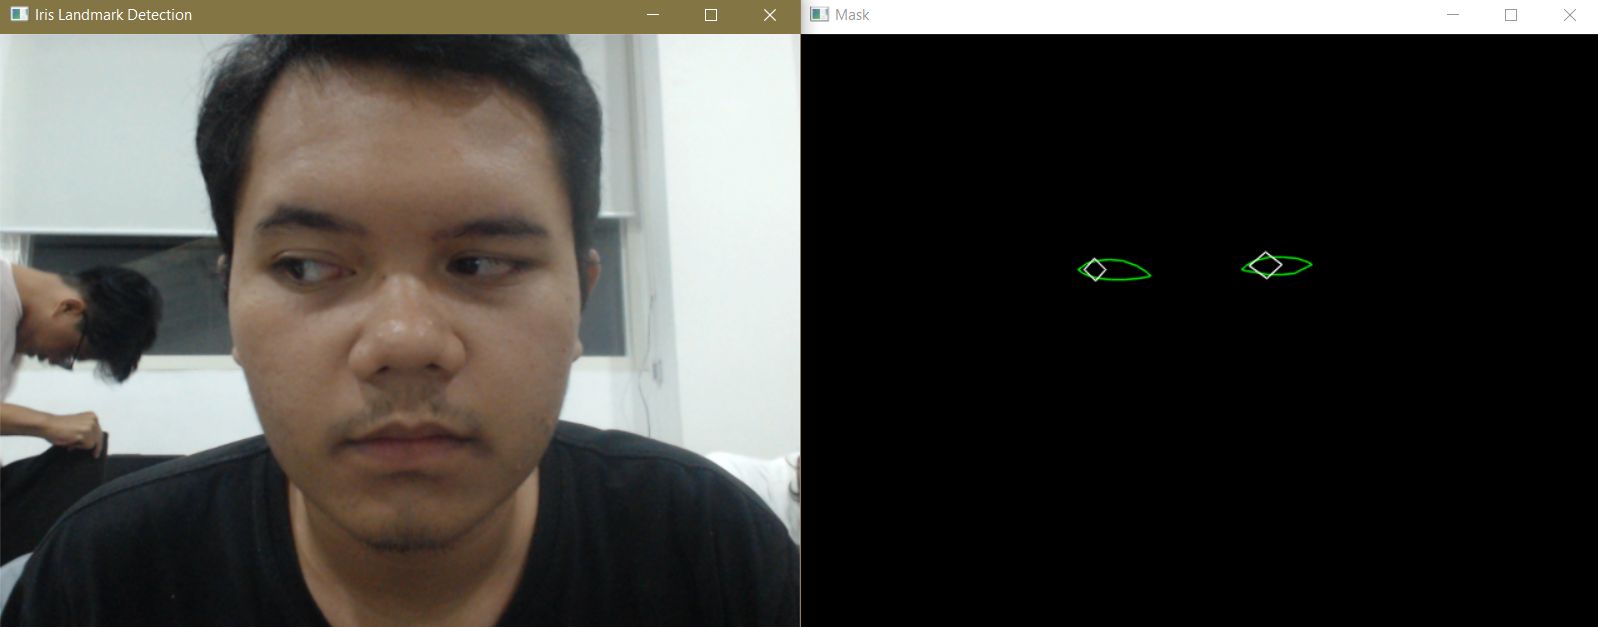
\includegraphics[scale=0.25]{gambar/bab3/kiri.png}   \\ \hline
        Maju               & 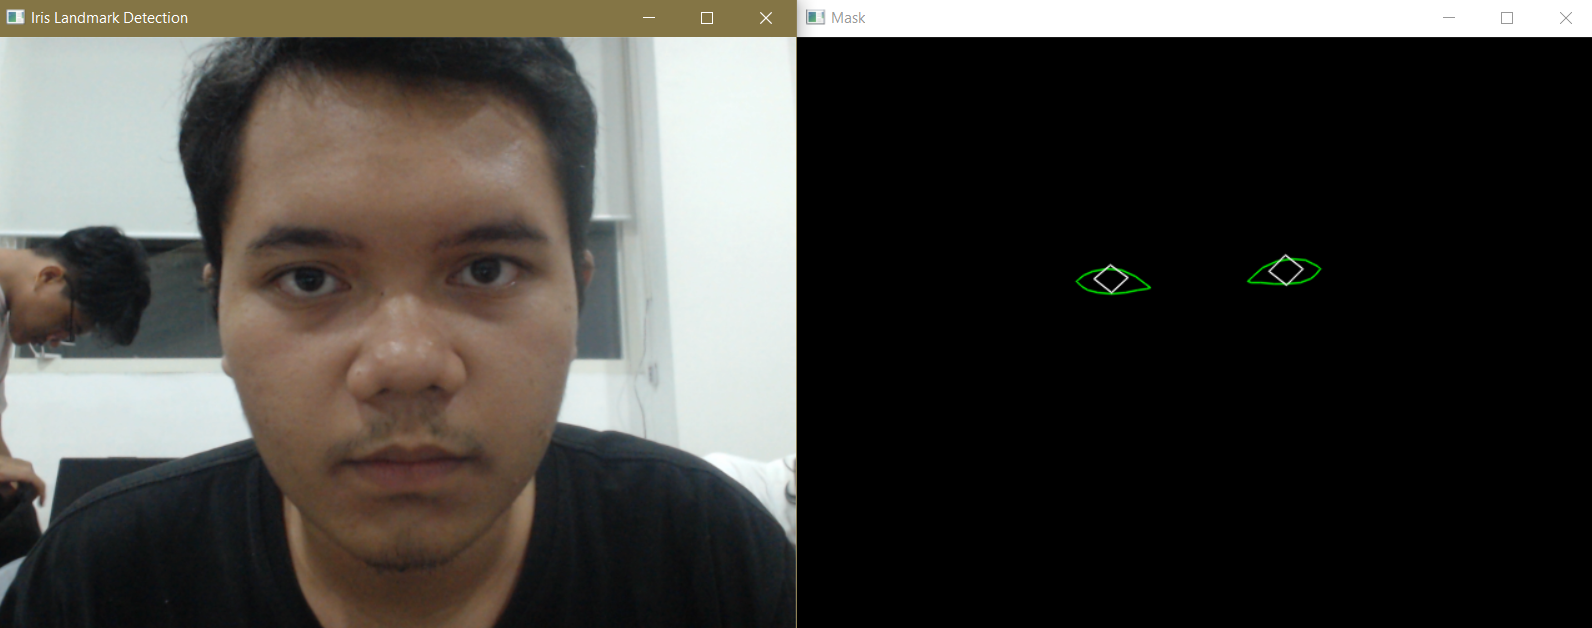
\includegraphics[scale=0.25]{gambar/bab3/maju.png}  \\ \hline
        Mundur               & 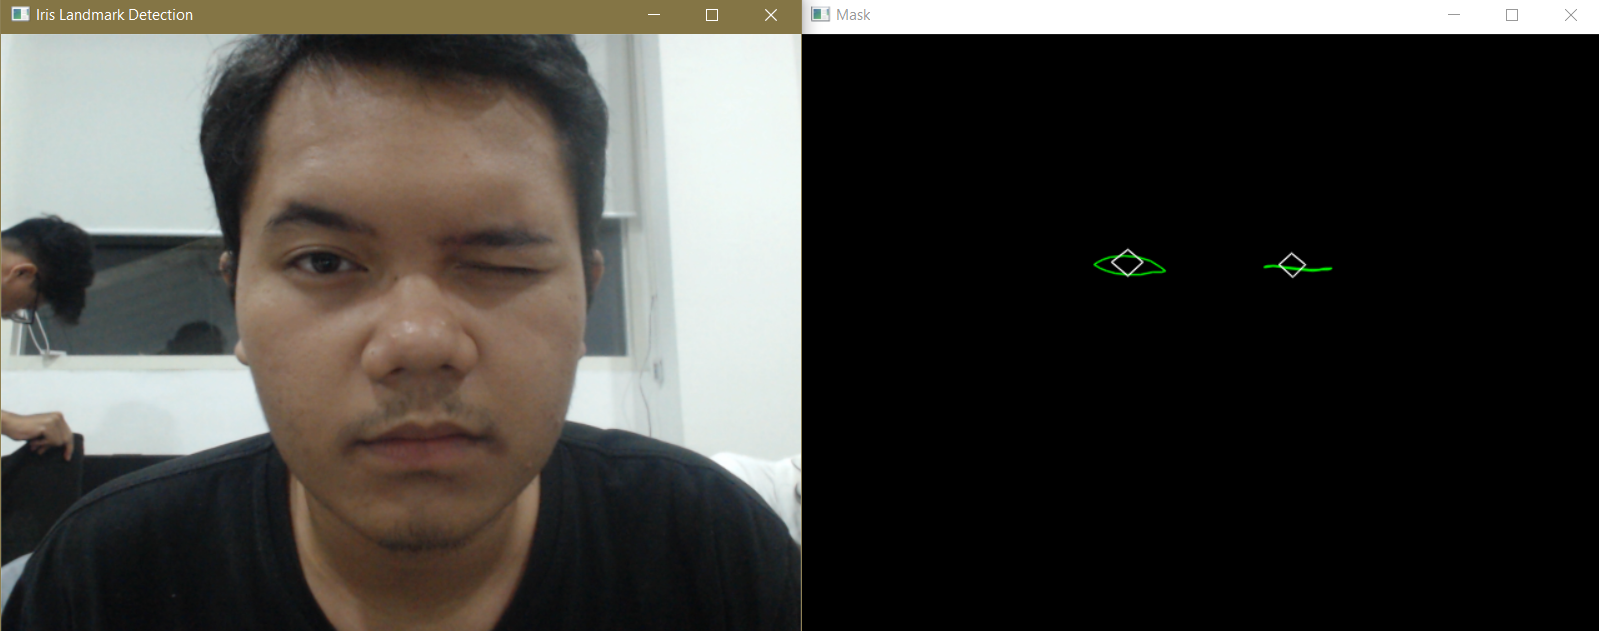
\includegraphics[scale=0.25]{gambar/bab3/mundur.png}  \\ \hline
        Stop               & 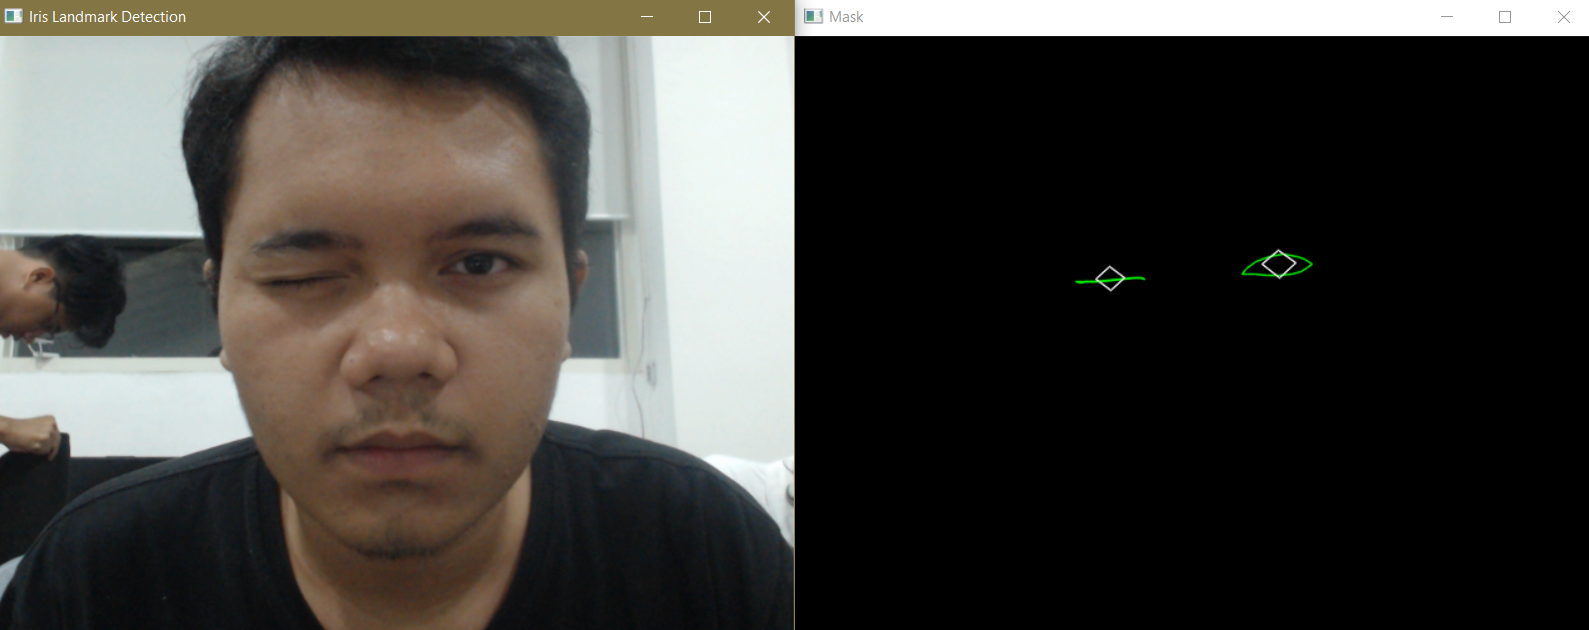
\includegraphics[scale=0.25]{gambar/bab3/stop.png}  \\ \hline
    \end{tabular}
\end{table}

\subsection{Optimasi Deteksi Mata}

Untuk meningkatkan performa dan akurasi, maka dataset ini kemudian akan melewati proses optimasi menggunakan algoritma \emph{Convolutional Neural Network} (CNN). Langkah ini melibatkan penyesuaian dan peningkatan model CNN untuk meningkatkan akurasi dan efisiensi dalam deteksi mata. Ini mungkin termasuk teknik seperti augmentasi data, tuning parameter, dsb. Penggunaan CNN dalam optimasi dataset diharapkan dapat menghasilkan model yang mampu mengenali pola dan fitur yang kompleks, sehingga sistem dapat memberikan respon yang tepat terhadap perubahan perintah yang diberikan oleh pengguna. Hasil dari model prediksi yang dibuat akan berupa h5.

\subsection{Implementasi ke NUC \textit{(Next Unit of Computing)}}

Setelah model CNN dioptimasi, langkah terakhir adalah implementasi model tersebut ke dalam NUC. Ini melibatkan integrasi kode, pengaturan lingkungan runtime, dan pengujian model pada perangkat NUC untuk mengontrol pergerakan kursi roda berbasis gestur mata.


%Section 3.2
\section{Bahan dan Peralatan yang Digunakan}

Untuk mendukung penelitian ini, perangkat kontrol, yang sudah dikembangkan, dibuat agar dapat menerima perintah secara nirkabel melalui perangkat lain seperti laptop maupun NUC. Sub bab ini menjelaskan implementasi alat yang dikembangkan dalam penelitian ini.

\subsection{\emph{Hardware} dan \emph{Software} yang Digunakan}
\label{sec:hardware dan software}

%List 3.1
Berikut beberapa \emph{Hardware} dan \emph{Software} yang digunakan dalam penelitian ini dijabarkan seperti berikut:
\begin{enumerate}
    \item Dataset Landmark Posisi Mata
    \item Kursi Roda Elektrik
    \item Laptop 
    \item Kamera
    \item Anaconda Navigator
    \item Visual Studio Code
    \item MediaPipe Face Mesh
    \item \textit{Convolutional Neural Network} (CNN)
    \item NUC \textit{(Next Unit of Computing)}

\end{enumerate}

\subsection{Alur Kerja Sistem}
\label{sec:alur kerja}

Pada penelitian ini dapat dibuat alur kerja sistem untuk menjelaskan lebih detail bagaimana proses antara \textit{software} dan \textit{hardware} dapat berinteraksi. 

%Gambar 3.5
\begin{figure} [ht] \centering
  % Nama dari file gambar yang diinputkan
  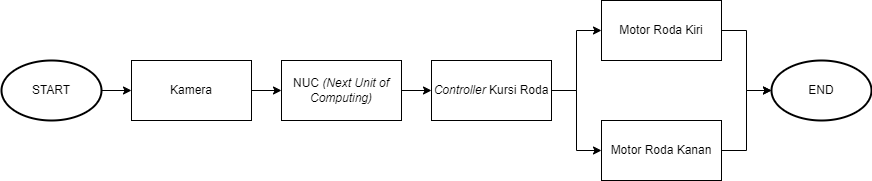
\includegraphics[scale=0.5]{gambar/bab3/hardware.png}
  % Keterangan gambar yang diinputkan
  \caption{Blok Diagram \textit{Hardware}}
  % Label referensi dari gambar yang diinputkan
  \label{fig:hardware}
\end{figure}

Berdasarkan alur kerja sistem di atas, pertama-tama, sistem menggunakan kamera yang dihubungkan dengan NUC \textit{(Next Unit of Computing)} sebagai perangkat utama untuk mendapatkan citra.

Setelah itu, citra akan diolah oleh MediaPipe Face Mesh untuk mendapatkan estimasi posisi mata. Kemudian, dari estimasi posiai mata, model CNN \textit{(Convolutional Neural Network)} akan mengklasifikasikan posisi mata. Setelah melakukan klasifikasi, software akan mengirim instruksi. Instruksi kemudian akan dikirim kepada \textit{controller} kursi roda yang nantinya digunakan sebagai petunjuk untuk mengatur gerakan pada motor roda kiri dan motor roda kanan pada kursi roda.